%!TEX root = slides.tex

\section{Algorithms}

\begin{frame}{Decision tree}
  \begin{description}
    \item[A decision tree] is a rooted tree where each vertex represents a decision.
    \vspace{4mm}
    \item[The results] of a decision are represented by the edges connecting the vertex to the vertices at the next level down.
    \vspace{4mm}
    \item[Decisions] can connect to other decisions further down the tree.
    \vspace{4mm}
    \item[Final outcomes] of the procedure are represented by the leaves.
  \end{description}
\end{frame}


\begin{frame}[fragile]{Decision tree for sorting three items}
  \begin{center}
    Three items -- $(\alpha, \beta, \gamma )$ \\[1cm]
    \begin{tikzpicture}[->,>=stealth',level/.style={sibling distance = 5cm/#1, level distance = 1.5cm}]
      \tikzset{every node/.style={align=center}}
      \node {\footnotesize $\alpha < \beta$}
        child { node {\footnotesize $\beta < \gamma$}
          child { node {\footnotesize $\alpha < \gamma$}
            child { node {\footnotesize $\alpha \beta \gamma$} edge from parent [->] node [left] {\tiny y} }
            child { node {\footnotesize $n/a$} edge from parent [->] node [right] {\tiny n} }
            edge from parent [->] node [left] {\tiny y} 
          } 
          child { node {\footnotesize $\alpha < \gamma$}
            child { node {\footnotesize $\alpha \gamma \beta$} edge from parent [->] node [left] {\tiny y} }
            child { node {\footnotesize $\gamma \alpha \beta$} edge from parent [->] node [right] {\tiny n} }
            edge from parent [->] node [right] {\tiny n} 
          }
          edge from parent [->] node [left] {\tiny y} 
        }
        child { node {\footnotesize $\beta < \gamma$}
          child { node {\footnotesize $\alpha < \gamma$}
            child { node {\footnotesize $\beta \alpha \gamma$} edge from parent [->] node [left] {\tiny y} }
            child { node {\footnotesize $n/a$} edge from parent [->] node [right] {\tiny n} }
            edge from parent [->] node [left] {\tiny y}
          }
          child { node {\footnotesize $\alpha < \gamma$}
            child { node {\footnotesize $\beta \gamma \alpha$} edge from parent [->] node [left] {\tiny y} }
            child { node {\footnotesize $\gamma \beta \alpha$} edge from parent [->] node [right] {\tiny n} }
            edge from parent [->] node [right] {\tiny n} 
          }
          edge from parent [->] node [right] {\tiny n} 
        };
			\end{tikzpicture}
  \end{center}
\end{frame}


\begin{frame}[fragile]{Decision tree for bubble sort with three items}
  \begin{center}
    Three items -- $(\alpha, \beta, \gamma )$ \\[1cm]
    \begin{tikzpicture}[->,>=stealth',level/.style={sibling distance = 5cm/#1, level distance = 1.5cm}]
      \tikzset{every node/.style={align=center}}
      \node {\footnotesize $x_1 < x_2$ \color{darkgray} ($\alpha \beta \gamma$)}
        child { node {\footnotesize $x_2 < x_3$ \color{darkgray} ($\alpha \beta \gamma$)}
          child { node {\footnotesize $x_1 < x_2$ \color{darkgray} ($\alpha \beta \gamma$)}
            child { node {\footnotesize $\alpha \beta \gamma$} edge from parent [->] node [left] {\tiny y} }
            child { node {\footnotesize $n/a$} edge from parent [->] node [right] {\tiny n} }
            edge from parent [->] node [left] {\tiny y} 
          } 
          child { node {\footnotesize $x_1 < x_2$ \color{darkgray} ($\alpha \gamma \beta$)}
            child { node {\footnotesize $\alpha \gamma \beta$} edge from parent [->] node [left] {\tiny y} }
            child { node {\footnotesize $\gamma \alpha \beta$} edge from parent [->] node [right] {\tiny n} }
            edge from parent [->] node [right] {\tiny n} 
          }
          edge from parent [->] node [left] {\tiny y} 
        }
        child { node {\footnotesize $x_2 < x_3$ \color{darkgray} ($\beta \alpha \gamma$)}
          child{ node {\footnotesize $x_1 < x_2$ \color{darkgray} ($\beta \alpha \gamma$)}
            child { node {\footnotesize $\beta \alpha \gamma$} edge from parent [->] node [left] {\tiny y} }
            child { node {\footnotesize $n/a$} edge from parent [->] node [right] {\tiny n} }
            edge from parent [->] node [left] {\tiny y} 
          }
          child { node {\footnotesize $x_1 < x_2$ \color{darkgray} ($\beta \gamma \alpha$)}
            child { node {\footnotesize $\beta \gamma \alpha$} edge from parent [->] node [left] {\tiny y} }
            child { node {\footnotesize $\gamma \beta \alpha$} edge from parent [->] node [right] {\tiny n} }
            edge from parent [->] node [right] {\tiny n} 
          }
          edge from parent [->] node [right] {\tiny n} 
        };
			\end{tikzpicture}
  \end{center}
\end{frame}


\begin{frame}{Heap sort}
  \begin{description}
    \item[Heap sort] uses a tree as part of the algorithm.
    \vspace{4mm}
    \item[This tree] is not a decision trees, it is for another purpose.
    \vspace{4mm}
    \item[Different] steps in the algorithm manipulate the tree.
    \vspace{4mm}
    \item[Worst case] -- performs better than quick sort.
    \vspace{4mm}
    \item[They have] the same average performance though.
  \end{description}
\end{frame}

\begin{frame}[fragile]{Heapsort initial tree}
  \begin{center}
    $(x_1,x_2,x_3,x_4,x_5,x_6,x_7,x_8,x_9,x_{10},x_{11},x_{12})$ \\[1cm]
    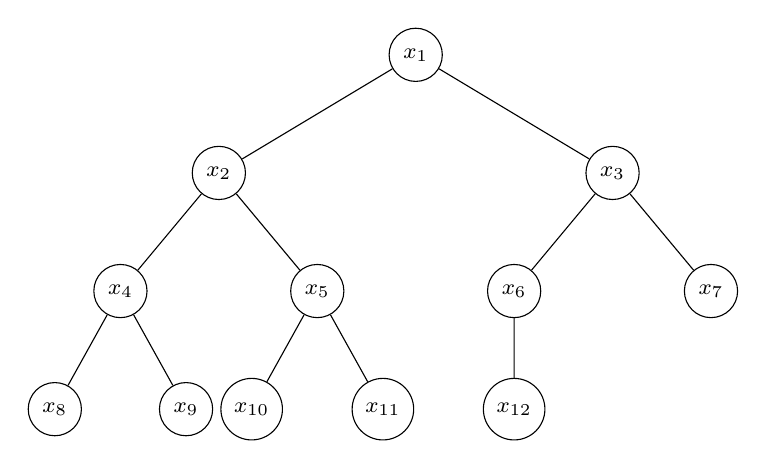
\begin{tikzpicture}[level/.style={sibling distance = 5cm/#1, level distance = 1.5cm}]
      \tikzset{every node/.style={align=center,draw,circle}}
      \node {\footnotesize $x_1$}
        child { node {\footnotesize $x_2$}
          child { node {\footnotesize $x_4$}
            child { node {\footnotesize $x_8$} }
            child { node {\footnotesize $x_9$} }
          } 
          child { node {\footnotesize $x_5$}
            child { node {\footnotesize $x_{10}$} }
            child { node {\footnotesize $x_{11}$} }
          }
        }
        child { node {\footnotesize $x_3$}
          child { node {\footnotesize $x_6$}
            child { node {\footnotesize $x_{12}$} }
          } 
          child { node {\footnotesize $x_7$} }
        };
			\end{tikzpicture}
  \end{center}
\end{frame}


\begin{frame}[fragile]{Heapsort initial tree}
  \begin{center}
    $(77,23,82,47,65,17,97,85,35,91,61,73)$ \\[1cm]
    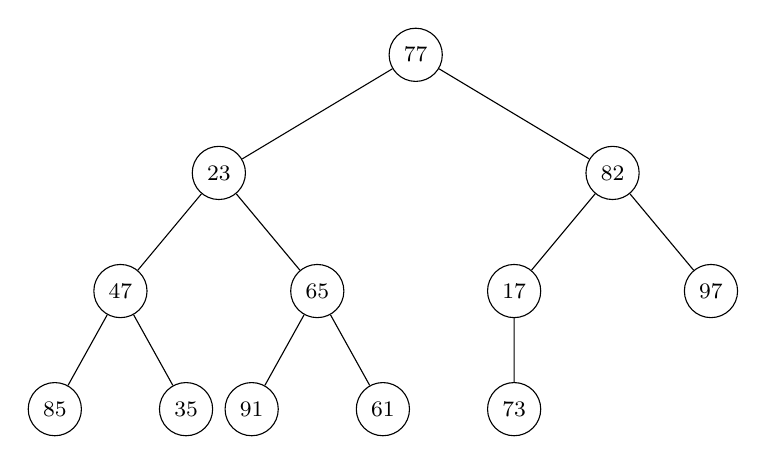
\begin{tikzpicture}[level/.style={sibling distance = 5cm/#1, level distance = 1.5cm}]
      \tikzset{every node/.style={align=center,draw,circle}}
      \node {\footnotesize $77$}
        child { node {\footnotesize $23$}
          child { node {\footnotesize $47$}
            child { node {\footnotesize $85$} }
            child { node {\footnotesize $35$} }
          } 
          child { node {\footnotesize $65$}
            child { node {\footnotesize $91$} }
            child { node {\footnotesize $61$} }
          }
        }
        child { node {\footnotesize $82$}
          child { node {\footnotesize $17$}
            child { node {\footnotesize $73$} }
          } 
          child { node {\footnotesize $97$} }
        };
			\end{tikzpicture}
  \end{center}
\end{frame}


\begin{frame}{Transforming to a heap}
  \begin{description}
    \item[Suppose] the trees at $x_{2r}$ and $x_{2r+1}$ are already heaps.
    \item[The vertex] $x_r$ is their parent.
    \item[Compare] $x_r$ to $x_{2r}$ and $x_{2r+1}$.
    \item[If] $x_r$ is smaller, do nothing.
    \item[Otherwise] replace $x_r$ with the smaller of it's children and fill the new vacancy with the smaller of $x_r$ and the two children, and repeat if necessary.
    \item[Start] this procedure at the last parent, and move backwards through the other parents.
  \end{description}
\end{frame}


\begin{frame}[fragile]{Heapsort - the heap}
  \begin{center}
    $(17,23,73,35,61,77,97,85,47,91,65,82)$ \\[2mm]
    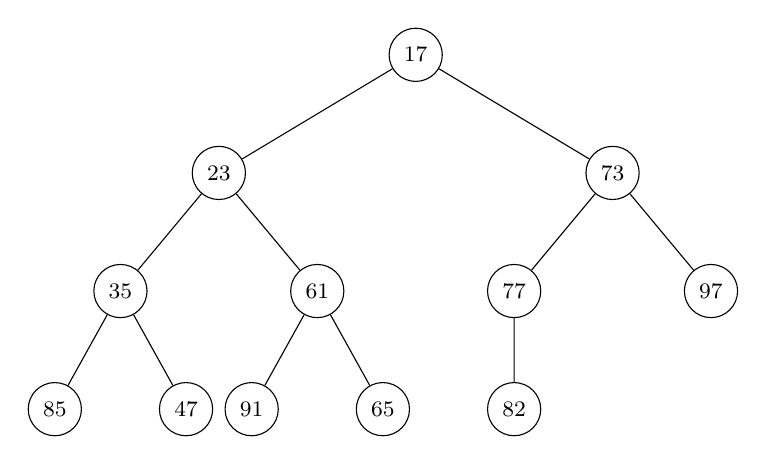
\begin{tikzpicture}[level/.style={sibling distance = 5cm/#1, level distance = 1.5cm}]
      \tikzset{every node/.style={align=center,draw,circle}}
      \node {\footnotesize $17$}
        child { node {\footnotesize $23$}
          child { node {\footnotesize $35$}
            child { node {\footnotesize $85$} }
            child { node {\footnotesize $47$} }
          } 
          child { node {\footnotesize $61$}
            child { node {\footnotesize $91$} }
            child { node {\footnotesize $65$} }
          }
        }
        child { node {\footnotesize $73$}
          child { node {\footnotesize $77$}
            child { node {\footnotesize $82$} }
          } 
          child { node {\footnotesize $97$} }
        };
    \end{tikzpicture} \\[2mm]
    $x_r < x_{2r}$ and $x_r < x_{2r+1}$
  \end{center}
\end{frame}


\begin{frame}{Transforming to a sorted list}
  \begin{description}
    \item[Start] with a new empty list.
    \item[Place] the root of the heap at the end of the list.
    \item[Remove] the last leaf and place it at the root.
    \item[Transform] the tree to a heap again. This is relatively easy since the subtrees at $x_2$ and $x_3$ are already heaps.
    \item[Repeat] from step 2.
  \end{description}
  \vspace{4mm}
  $$ (17,23,35,47,61,65,73,77,82,85,91,97) $$
\end{frame}
